%-------------------------------------------------------------------------
% td-info-S1-fonctions.tex
%-------------------------------------------------------------------------

\begin{td}[Codage des entiers positifs (1)]\label{td:codageEntier}\index[td]{codage des entiers positifs}
\em
Définir un algorithme qui code sur $k$ chiffres en base $b$ un entier positif 
$n$ du système décimal.

Exemples : 
$\begin{array}[t]{l@{\rightarrow}l}
(38)_{10} & (123)_{5} \\
(83)_{10} & (123)_{8} \\
(291)_{10} & (123)_{16}
\end{array}$
\end{td}

\begin{td}[Codage d'un nombre fractionnaire]\label{td:fraction}\index[td]{codage d'un nombre fractionnaire}
\em
Un nombre fractionnaire ({\em nombre avec des chiffres après la virgule} :
{$(r_nr_{n-1}\ldots r_1r_0.r_{-1}r_{-2}\ldots)_b$})
est défini sur un sous-en\-semble borné, incomplet et fini des rationnels.
Un tel nombre a pour valeur :
$${r_nb^n + r_{n-1}b^{n-1} + \ldots + r_1b^1 + r_0b^0 + r_{-1}b^{-1} + r_{-2}b^{-2} + \ldots}$$
En pratique, le {\em nombre de chiffres après la virgule} est limité par la taille physique
en machine.
$${(r_nr_{n-1}\ldots r_1r_0.r_{-1}r_{-2}\ldots r_{-k})_b = \sum_{i=-k}^{i=n} r_ib^i}$$
Un nombre $x$ pourra être représenté en base $b$ par un triplet
$[s,m,p]$ tel que ${x = (-1)^s \cdot m \cdot b^p}$ où $s$ représente le signe de $x$,
$m$ sa mantisse et $p$ son exposant ($p$ comme puissance) où :
\begin{itemize}
\item signe $s$ : $s = 1$ si $x < 0$ et $s = 0$ si $x \geq 0$
\item mantisse $m$ : $m \in [1,b[$ si $x \neq 0$ et $m = 0$ si $x = 0$
\item exposant $p$ : $p \in [min,max]$
\end{itemize}
Ainsi, le codage de $x = -9.75$ en base $b = 2$ s'effectuera en 4
étapes :
\begin{enumerate}
\item coder le signe de $x$ : $x = -9.75 < 0 \Rightarrow {s = 1}$
\item coder la partie entière de $|x|$ : {$9 = (1001)_2$}
\item coder la partie fractionnaire de $|x|$ : {$0.75 = (0.11)_2$}
\item et coder $|x|$ en notation scientifique normalisée : $m \in [1,2[$\\
	$(1001)_2 + (0.11)_2 = (1001.11)_2 = (1.00111)_2\cdot 2^{3}$\\ 
	$= {(1.00111)_2\cdot 2^{{(11)}_2}}$
\end{enumerate}
Cette démarche en 4 étapes conduit au résultat $x = (-1)^s \cdot m \cdot b^p = (-1)^{1} \cdot (1.00111)_2 \cdot 2^{(11)_2}$ où
$b = 2$, $s = (1)_2$, $m = (1.00111)_2$  et $p = (11)_2$.

Déterminer le signe, la mantisse et l'exposant binaires 
du nombre fractionnaire $x = 140.8125$ 
en suivant les 4 étapes décrites ci-dessus.
\end{td}


\begin{td}[Décodage base b $\rightarrow$ décimal]\label{td:decoder}\index[td]{décodage base b $\rightarrow$ décimal}
\em
La valeur décimale d'un nombre entier
codé en base $b$ peut être obtenue par l'algorithme suivant :\\
{\tt \mbox{}\ \ \ \ }\begin{py}{7.5cm}\tt
>>> n = 0\\
>>> for i in range(len(code)):\\
...     n = n + code[i]*b**(len(code)-1-i)\\
... \\
>>> 
\end{py}\\[1mm]
Spécifier une fonction qui encapsulera cet algorithme.
\end{td}

\begin{td}[Codage des entiers positifs (2)]\label{td:codage}\index[td]{codage des entiers positifs}
\em
Définir (spécifier et implémenter) une fonction qui 
code un entier $n$ en base $b$ sur $k$ chiffres
(voir TD \ref{td:codageEntier}).
\end{td}

\begin{td}[Une spécification, des implémentations]\label{td:implem}\index[td]{spécification et implémentations}
\em
\begin{enumerate}
\item Proposer deux implémentations du calcul de
la somme $s = \sum_0^n u_k$ des $n$ premiers termes d'une suite 
géométrique $u_k = a\cdot b^k$.
\item Comparer les complexités de ces deux im\-plé\-men\-ta\-tions.
\end{enumerate}
\end{td}

\begin{td}[Passage par valeur]\label{td:swap}\index[td]{passage par valeur}
\em
On considère les codes suivants :

{\tt \mbox{}\ }\begin{py}{2.25cm}\tt
>>> x, y\\
(1, 2)\\
>>> tmp = x\\
>>> x = y\\
>>> y = tmp\\
>>> x, y\\
(2, 1)
\end{py}
\hfill
\begin{py}{3cm}\tt
def swap(x,y):\\
\mbox{}\ \ \ \ tmp = x\\
\mbox{}\ \ \ \ x = y\\
\mbox{}\ \ \ \ y = tmp\\
\mbox{}\ \ \ \ return
\end{py}
\hfill
\begin{py}{2.25cm}\tt
>>> x, y\\
(1, 2)\\
>>> swap(x,y)\\
>>> x, y\\
(1, 2)
\end{py}\\[1mm]
Expliquer la différence entre l'exécution de gauche et l'exécution de droite
en explicitant l'appel équivalent à l'appel {\tt swap(x,y)} dans l'exécution
de droite.
\end{td}

\begin{td}[Valeurs par défaut]\label{td:defaut}\index[td]{valeurs par défaut}
\em
On considère la fonction qui code en base $b$ sur $k$ chiffres
un nombre décimal $n$ (voir TD \ref{td:codage}). 
Proposer une définition de cette fonction où $k = 8$ et $b = 2$ par défaut.
\end{td}

\begin{td}[Portée des variables]\label{td:portee}\index[td]{portée des variables}
\em
On considère les fonctions {\tt f}, {\tt g} et {\tt h} suivantes :

\begin{py}{2.5cm}\tt
def f(x):\\
\mbox{}\ \ x = 2*x\\
\mbox{}\ \ print('f', x)\\
\mbox{}\ \ return x
\end{py}
\hfill
\begin{py}{2.5cm}\tt
def g(x):\\
\mbox{}\ \ x = 2*f(x)\\
\mbox{}\ \ print('g', x)\\
\mbox{}\ \ return x
\end{py}
\hfill
\begin{py}{2.5cm}\tt
def h(x):\\
\mbox{}\ \ x = 2*g(f(x))\\
\mbox{}\ \ print('h', x)\\
\mbox{}\ \ return x
\end{py}
\mbox{}\vspace*{2mm}

Qu'affichent les appels suivants ?\\
\mbox{}\\
\begin{minipage}{3.5cm}
\begin{enumerate}
\item 
\begin{py}{2.5cm}\tt
>>> x = 5\\
>>> print(x)\\
{\color{red} ?}\\
>>> y = f(x)\\
>>> print(x)\\
{\color{red} ?}\\
>>> z = g(x)\\
>>> print(x)\\
{\color{red} ?}\\
>>> t = h(x)\\
>>> print(x)\\
{\color{red} ?}
\end{py}
\end{enumerate}
\end{minipage}
\hfill
\begin{minipage}{3.5cm}
\begin{enumerate}\setcounter{enumi}{1}
\item 
\begin{py}{2.5cm}\tt
>>> x = 5\\
>>> print(x)\\
{\color{red} ?}\\
>>> x = f(x)\\
>>> print(x)\\
{\color{red} ?}\\
>>> x = g(x)\\
>>> print(x)\\
{\color{red} ?}\\
>>> x = h(x)\\
>>> print(x)\\
{\color{red} ?}
\end{py}
\end{enumerate}
\end{minipage}
\end{td}


\begin{td}[Tours de Hanoï {\em à la main}]\label{td:hanoi}\index[td]{tours de Hanoï}
\em
Résoudre {\em à la main} le problème des tours de Hanoï à $n$ disques
(voir figure \ref{fig:hanoi}) successivement 
pour $n=1$, $n=2$, $n=3$ et $n=4$.
\end{td}
\begin{fig}[Tours de Hanoï (1)]\label{fig:hanoi}
{\bf Etat initial :}\\
\centerline{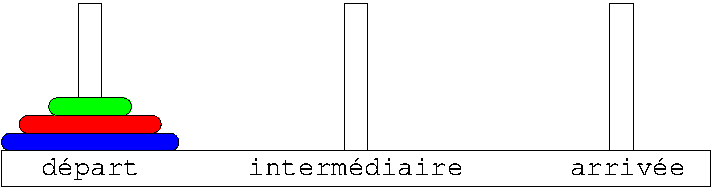
\includegraphics[width=6cm]{hanoi.pdf}}

\noindent{\bf Etat final :}\\
\centerline{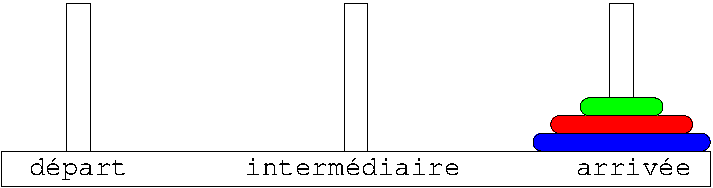
\includegraphics[width=6cm]{hanoi1.pdf}}
\end{fig}



\begin{td}[Pgcd et ppcm de 2 entiers (1)]\label{td:pgcd}\index[td]{pgcd et ppcm de 2 entiers}
\em
\begin{enumerate}
\item Définir une fonction récursive qui calcule le plus grand commun 
	diviseur $d$ de 2 entiers $a$ et $b$ : \\
	$\rm{pgcd}(a,b) = \rm{pgcd}(b,a \bmod b) = \ldots = \rm{pgcd}(d,0) = d$.
\item En déduire une fonction qui calcule le plus petit commun multiple $m$ de 2 entiers $a$ et $b$.
\end{enumerate}
\end{td}

\begin{td}[Somme arithmétique]\label{td:somme}\index[td]{suite arithmétique}
\em
\begin{enumerate}
\item Définir une fonction récursive qui calcule la somme des $n$ premiers
	nombres entiers.
	$$s = \sum^{n}_{k=0}k = \frac{n(n+1)}{2}$$
\item Comparer la complexité de cette version avec les versions constante
	et itérative (voir TD \ref{td:implem}).
\end{enumerate}
\end{td}

\begin{td}[Courbes fractales]\label{td:fractal}\index[algo]{courbes fractales}\index[td]{courbes fractales}
\em
On s'intéresse ici aux programmes dont l'exécution produit des dessins
à l'aide de la tortue Logo.
On consid\`ere la proc\'edure {\tt draw} ci-dessous :

\mbox{}\ \ \begin{py}{7cm}\tt
def draw(n,d):\\
\mbox{}\ \ \ \ assert type(n) is int\\
\mbox{}\ \ \ \ assert n >= 0\\
\mbox{}\ \ \ \ if n == 0: forward(d)\\
\mbox{}\ \ \ \ else:\\
\mbox{}\ \ \ \ \ \ \ \ draw(n-1,d/3.)\\
\mbox{}\ \ \ \ \ \ \ \ left(60)\\
\mbox{}\ \ \ \ \ \ \ \ draw(n-1,d/3.)\\
\mbox{}\ \ \ \ \ \ \ \ right(120)\\
\mbox{}\ \ \ \ \ \ \ \ draw(n-1,d/3.)\\
\mbox{}\ \ \ \ \ \ \ \ left(60)\\
\mbox{}\ \ \ \ \ \ \ \ draw(n-1,d/3.)\\
\mbox{}\ \ \ \ return
\end{py}\\[1mm]
Dessiner le résultat des appels {\tt draw(n,900)} respectivement pour {\tt n = 0},
	{\tt n = 1}, {\tt n = 2} et {\tt n = 3}. A chaque appel, le crayon est 
	initialement en $(0,0)$ avec une direction de $0$.
\end{td}

\begin{td}[QCM (3)]\label{td:qcm3}\index{evaluation@évaluation!contrôle d'attention}
\index{fonction!qcm}\index[td]{contrôle d'attention} (un seul item correct par question)
\em
\begin{enumerate}
\item La réutilisabilité d'un algorithme est son aptitude
	\begin{enumerate}
	\item à utiliser de manière optimale les ressources du matériel qui l'exécute
	\item à se protéger de conditions anormales d'utilisation
	\item à résoudre des tâches équivalentes à celle pour laquelle il a été conçu
	\item à réaliser exactement la tâche pour laquelle il a été conçu
	\end{enumerate}

\item L'encapsulation est l'action
	\begin{enumerate}
	\item de mettre une chose dans une autre
	\item de fermer une chose par une autre
	\item de substituer une chose par une autre
	\item de remplacer une chose par une autre
	\end{enumerate}
	
\item Une fonction est un bloc d'instructions nommé et paramétré 
	\begin{enumerate}
	\item qui ne peut pas retourner plusieurs valeurs
	\item qui ne peut pas contenir d'instructions itératives
	\item qui retourne une valeur
	\item qui ne retourne pas de valeur
	\end{enumerate}

\item Les paramètres d'entrée d'une fonction sont
	\begin{enumerate}
	\item les arguments nécessaires pour effectuer le traitement associé à la fonction
	\item les valeurs obtenues après avoir effectué le traitement associé à la fonction
	\item des grandeurs invariantes pendant l'exécution de la fonction
	\item des variables auxiliaires définies dans le corps de la fonction
	\end{enumerate}
	
\item Les préconditions d'une fonction sont des conditions à respecter 
	\begin{enumerate}
	\item par les paramètres de sortie de la fonction
	\item pendant toute l'exécution de la fonction
	\item par les paramètres d'entrée de la fonction
	\item pour pouvoir compiler la fonction
	\end{enumerate}
	
\item La description d'une fonction décrit
	\begin{enumerate}
	\item ce que fait la fonction
	\item comment fait la fonction
	\item pourquoi la fonction le fait 
	\item où la fonction le fait
	\end{enumerate}
	
\item Le jeu de tests d'une fonction est 
	\begin{enumerate}
	\item un ensemble d'exercices à résoudre
	\item un ensemble d'exceptions dans le fonctionnement de la fonction
	\item un ensemble caractéristiques d'entrées-sorties associées
	\item un ensemble de recommandations dans l'utilisation de la fonction
	\end{enumerate}

\item En {\sc Python}, l'instruction {\tt assert} permet de 
	\begin{enumerate}
	\item tester une précondition
	\item imposer une instruction
	\item paramétrer une fonction
	\item tester un test du jeu de tests
	\end{enumerate}

\item La validité d'une fonction est son aptitude à réaliser exactement 
	la tâche pour laquelle elle a été conçue. Plus concrètement,
	\begin{enumerate}
	\item la fonction doit vérifier impérativement ses préconditions
	\item la fonction doit être correctement paramétrée
	\item l'implémentation de la fonction doit être conforme aux jeux de tests
	\item l'utilisation de la fonction doit être conviviale
	\end{enumerate}

\item Le passage des paramètres par valeur consiste à copier
	\begin{enumerate}
	\item la valeur du paramètre formel dans le paramètre effectif correspondant
	\item la référence du paramètre effectif dans le paramètre formel correspondant
	\item la référence du paramètre formel dans le paramètre effectif correspondant
	\item la valeur du paramètre effectif dans le paramètre formel correspondant
	\end{enumerate}
	
\item Un appel récursif est un appel 
	\begin{enumerate}
	\item dont l'exécution est un processus récursif
	\item dont l'exécution est un processus itératif
	\item dont le résultat est retourné par la fonction
	\item d'une fonction par elle-même
	\end{enumerate}	
\end{enumerate}
\end{td}


\begin{td}[Passage des paramètres]\label{td:passage}\index{fonction!passage par valeur}\index[td]{passage par valeur}
\em
On considère les fonctions {\tt f}, {\tt g} et {\tt h} suivantes :

\begin{center}
\begin{py}{4cm}
\begin{verbatim}
def f(x):
    y = x + 2
    return y
\end{verbatim}
\end{py}\hspace*{1cm}
\begin{py}{4cm}
\begin{verbatim}
def g(z):
    v = 2*f(z)
    return v
\end{verbatim}
\end{py}\hspace*{1cm}
\begin{py}{4cm}
\begin{verbatim}
def h(a):
    b = g(f(a))
    return b
\end{verbatim}
\end{py}
\end{center}

Quels sont les algorithmes équivalents (algorithmes où il n'y a plus 
d'appels aux fonctions {\tt f}, {\tt g} et {\tt h}) aux appels suivants :
\vspace*{2mm}

\begin{minipage}{4cm}
\begin{enumerate}
\item {\tt u = f(2)}
\item {\tt u = f(t)}
\end{enumerate}
\end{minipage}\hfill
\begin{minipage}{4cm}
\begin{enumerate}\setcounter{enumi}{2}
\item {\tt u = g(2)}
\item {\tt u = g(t)}
\end{enumerate}
\end{minipage}\hfill
\begin{minipage}{4cm}
\begin{enumerate}\setcounter{enumi}{4}
\item {\tt u = h(2)}
\item {\tt u = h(t)}
\end{enumerate}
\end{minipage}

\end{td}

\begin{td}[Portée des variables (2)]\label{td:portee2}\index{variable!portée}\index[td]{portée des variables}
\em
On considère les fonctions {\tt f}, {\tt g} et {\tt h} suivantes :
\begin{center}
\begin{py}{4cm}
\begin{verbatim}
def f(x):
    x = x + 2
    print('f', x)
    return x
\end{verbatim}
\end{py}\hspace*{1cm}
\begin{py}{4cm}
\begin{verbatim}
def g(x):
    x = 2*f(x)
    print('g', x)
    return x
\end{verbatim}
\end{py}\hspace*{1cm}
\begin{py}{4cm}
\begin{verbatim}
def h(x):
    x = g(f(x))
    print('h', x)
    return x
\end{verbatim}
\end{py}
\end{center}

Qu'affichent les appels suivants ?
\vspace*{2mm}

\begin{minipage}[t]{7cm}
\begin{enumerate}
\item 

\begin{py}{4cm}
\begin{verbatim}
>>> x = 5
>>> print(x)

>>> x = x + 2
>>> print(x)

>>> x = 2 * (x + 2)
>>> print(x)

\end{verbatim}
\end{py}

\item 

\begin{py}{4cm}
\begin{verbatim}
>>> x = 5
>>> print(x)

>>> y = f(x)
>>> print(x, y)

>>> z = 2*f(y)
>>> print(x, y, z)

\end{verbatim}
\end{py}


\item 

\begin{py}{4cm}
\begin{verbatim}
>>> x = 5
>>> print(x)

>>> z = 2*f(f(x))
>>> print(x, z)

\end{verbatim}
\end{py}


\end{enumerate}
\end{minipage}\hfill
\begin{minipage}[t]{7cm}
\begin{enumerate}\setcounter{enumi}{3}
\item 

\begin{py}{4cm}
\begin{verbatim}
>>> x = 5
>>> print(x)

>>> f(x)

>>> print(x)

>>> g(x)

>>> print(x)

>>> h(x)

>>> print(x)

\end{verbatim}
\end{py}


\end{enumerate}
\end{minipage}
\end{td}


\begin{td}[Suite géométrique]\label{td:geometrie}\index[algo]{suites numériques}\index[td]{suite
géométriques}
\em
Définir une fonction récursive qui calcule la somme des $n$ premiers termes 
d'une suite géométrique $u_k = ab^k$.
\end{td}

\begin{td}[Puissance entière]\label{td:puissance}\index[algo]{fonction puissance}\index[td]{fonction puissance}
\em
Définir une fonction récursive qui calcule la puissance entière $p = x^n$ 
d'un nombre entier $x$.
\end{td}

\begin{td}[Coefficients du binôme]\label{td:binome}\index[algo]{coefficients du binôme}\index[td]{coefficients du binôme}
\em
Définir une fonction récursive qui calcule les coefficients du binôme :\\
$\displaystyle (a+b)^n = \sum_{k=0}^n \frac{n!}{k!(n-k)!}a^{n-k}b^k$.
\end{td}

\begin{td}[Fonction d'Ackerman]\label{td:ackerman}\index[algo]{fonction d'Ackerman}\index[td]{fonction d'Ackerman}\index{{{\sc Ackerman}}}
\em
Définir une fonction récursive qui calcule la fonction d'Ackerman : 
$$
{f : N^2 \rightarrow N}\ 
\left\{\begin{array}{lll}
f{(0,n)} & = & n+1\\
f{(m,0)} & = & f{(m-1,1)}\mbox{\ si\ } m > 0\\
f{(m,n)} & = & f{(m-1,f{(m,n-1)})}\mbox{\ si\ } m > 0, n > 0
\end{array}\right.
$$
\end{td}

\begin{td}[Addition binaire]\label{td:addition2}\index[algo]{opérations binaires}\index[td]{addition binaire}
\em
Définir une fonction {\tt add2} qui effectue l'addition binaire de 2 
entiers $a$ et $b$ (le nombre de bits n'est pas limité {\em a priori}).\\
Exemple : $(0101)_2 + (10011)_2 = (11000)_2$

\begin{py}{7cm}
\begin{verbatim}
# add2(a,b)
>>> add2([1,0],[1,0,1,1])
[1, 1, 0, 1]
>>> add2([1,0,1,1],[1,0])
[1, 1, 0, 1]
>>> add2([1,1],[1,1])
[1, 1, 0]
\end{verbatim}
\end{py}
\end{td}

\begin{td}[Complément à 2]\label{td:complement2}\index[td]{complément à 2}
\em
Définir une fonction {\tt neg2} qui détermine le complément à 2 en binaire 
d'un entier $n$ codé sur $k$ bits.
	$$(011100)_2 \rightarrow (100100)_2\ :\ \begin{array}[t]{lrr} 
	  & (011100)_2\\
	\hline
	  & (100011)_2\\
	+ & (000001)_2\\
	\hline
	= & (100100)_2
	\end{array}$$

	\begin{py}{7cm}
	\begin{verbatim}
	# neg2(code)
	>>> neg2([0,0,0,1,0,1,1,1])
	[1, 1, 1, 0, 1, 0, 0, 1]
	>>> neg2([1, 1, 1, 0, 1, 0, 0, 1])
	[0, 0, 0, 1, 0, 1, 1, 1]
	>>> for a in [0,1]:
	...    for b in [0,1]:
	...        for c in [0,1]:
	...            add2([a,b,c],neg2([a,b,c]))
	[0, 0, 0]
	[1, 0, 0, 0]
	[1, 0, 0, 0]
	[1, 0, 0, 0]
	[1, 0, 0, 0]
	[1, 0, 0, 0]
	[1, 0, 0, 0]
	[1, 0, 0, 0]
	\end{verbatim}
	\end{py}
\end{td}

\begin{td}[Codage-décodage des réels]\label{td:ieee754}\index[algo]{codage des réels}\index[td]{codage des réels}\index{norme IEEE 754}
\em

\begin{enumerate}
\item Définir une fonction {\tt ieee} qui code
	un nombre réel $x$ selon la norme IEEE 754 simple précision.
	$$x = (-1)^s\cdot (1+m)\cdot 2^{(e-127)}$$

	\begin{py}{7cm}
	\begin{verbatim}
	# ieee(x)
	>>> ieee(0.0)
	[0, 0, 0, 0, 0, 0, 0, 0, 0, 
	 0, 0, 0, 0, 0, 0, 0, 0, 0, 0, 0, 
	 0, 0, 0, 0, 0, 0, 0, 0, 0, 0, 0, 0]
	>>> ieee(0.625)
	[0, 0, 1, 1, 1, 1, 1, 1, 0, 
	 0, 1, 0, 0, 0, 0, 0, 0, 0, 0, 0, 
	 0, 0, 0, 0, 0, 0, 0, 0, 0, 0, 0, 0]
	>>> ieee(3.1399998664855957)
	[0, 1, 0, 0, 0, 0, 0, 0, 0, 
	 1, 0, 0, 1, 0, 0, 0, 1, 1, 1, 1, 
	 0, 1, 0, 1, 1, 1, 0, 0, 0, 0, 1, 0]
	>>> ieee(-4573.5)
	[1, 1, 0, 0, 0, 1, 0, 1, 1, 
	 0, 0, 0, 1, 1, 1, 0, 1, 1, 1, 0, 
	 1, 1, 0, 0, 0, 0, 0, 0, 0, 0, 0, 0]
	\end{verbatim}
	\end{py}

\item Définir une fonction {\tt real} qui décode un nombre réel $x$ 
	codé selon la norme IEEE 754 simple précision.
	$$x = (-1)^s\cdot (1+m)\cdot 2^{(e-127)}$$

	\begin{py}{7cm}
	\begin{verbatim}
	# real(code)
	>>> real(ieee(0.625))
	0.625
	>>> real(ieee(3.1399998664855957))
	3.1399998664855957
	>>> real(ieee(-4573.5))
	-4573.5
	\end{verbatim}
	\end{py}
\end{enumerate}

\noindent On pourra vérifier les résultats obtenus avec la fonction {\tt ieee}
du TD \ref{td:ieee754} ci-contre sur le site 
\href{http://babbage.cs.qc.edu/IEEE-754/Decimal.html}{\tt http\char`://babbage.cs.qc.edu/IEEE-754/Decimal.html}

\end{td}

\begin{td}[Intégration numérique]\label{td:integration}\index[algo]{intégration numérique}\index[td]{intégration numérique}
\em
Soit $f(x)$ une fonction continue de $R \rightarrow R$ à intégrer sur $[a,b]$ 
(on supposera que $f$ à toutes les bonnes propriétés mathématiques pour être
intégrable sur l'intervalle considéré). On cherche à calculer son intégrale
$\displaystyle I = \int_a^b f(x)dx$ qui représente classiquement l'aire
comprise entre la courbe représentative de $f$ et les droites d'équations 
$x=a$, $x=b$ et $y=0$. Les méthodes d'intégration numérique (méthode des rectangles, 
méthode des trapèzes et méthode de Simpson) consistent 
essentiellement à trouver une bonne approximation de cette aire.
$$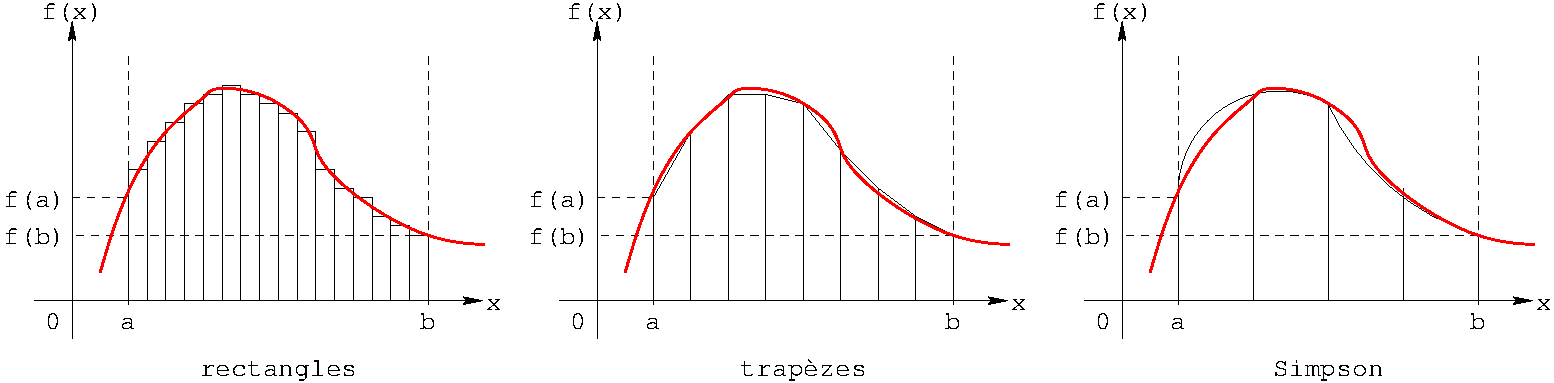
\includegraphics[width=14cm]{integrale.pdf}$$

On testera ces différentes méthodes avec la fonction $f(x) = \sin(x)$ sur $[0,\pi]$.
\begin{enumerate}
\item Méthode des rectangles : subdivisons l'intervalle d'intégration de
	longueur $b-a$ en $n$ parties égales de longueur 
	$\displaystyle\Delta x = \frac{b-a}{n}$. Soient $x_1$, $x_2$, \ldots,
	$x_n$ les points milieux de ces $n$ intervalles. Les $n$ rectangles
	formés avec les ordonnées correspondantes ont pour surface $f(x_1)\Delta
	x$, $f(x_2)\Delta x$, \ldots, $f(x_n)\Delta x$. L'aire sous la courbe 
	est alors assimilée à la somme des aires de ces rectangles, soit 
	$$\displaystyle I = \int_a^b f(x)dx \approx
	\left(f(x_1)+f(x_2)+\cdots+f(x_n)\right)\Delta x$$ 
	C'est la formule dite
	des rectangles qui repose sur une approximation par une fonction {\em en
	escalier}.
	
	Ecrire une fonction {\tt rectangle\_integration} qui calcule l'intégrale définie $I$ d'une fonction 
	$f$ sur $[a,b]$ à l'ordre $n$ par la méthode des rectangles.
	
\item Méthode des trapèzes : subdivisons l'intervalle d'intégration de
	longueur $b-a$ en $n$ parties égales de longueur 
	$\displaystyle\Delta x = \frac{b-a}{n}$. Les abscisses des points ainsi
	définis sont
	$a$, $x_1$, $x_2$, \ldots, $x_{n-1}$, $b$ et les trapèzes construits sur ces
	points et les ordonnées correspondantes ont pour aire 
	$\displaystyle \frac{\Delta x}{2}\left(f(a) + f(x_1)\right)$,
	$\displaystyle \frac{\Delta x}{2}\left(f(x_1) + f(x_2)\right)$,
	\ldots,
	$\displaystyle \frac{\Delta x}{2}\left(f(x_{n-1}) + f(b)\right)$.
	L'aire sous la courbe est alors assimilée à la somme des aires de ces 
	trapèzes, soit
	$$\displaystyle I = \int_a^b f(x)dx \approx
	\left(\frac{f(a)+f(b)}{2} + f(x_1) + f(x_2) + \cdots + f(x_{n-1})\right)
	\Delta x$$
	C'est la formule dite des trapèzes.
	
	Ecrire une fonction {\tt trapezoid\_integration} qui calcule l'intégrale définie $I$ d'une fonction 
	$f$ sur $[a,b]$ à l'ordre $n$ par la méthode des trapèzes.
	
\item Méthode de Simpson : divisons l'intervalle d'intégration $[a,b]$ en un nombre 
	$n$ pair d'inter\-val\-les dont la longueur est 
	$\displaystyle\Delta x = \frac{b-a}{n}$. 
	Dans les 2 premiers intervalles d'extrémités $a$, $x_1$ et $x_2$, on approche 
	la courbe représentative de $f$ par une parabole d'équation 
	$y = \alpha x^2 + \beta x + \gamma$ passant par les points $A(a,f(a))$, 
	$A_1(x_1,f(x_1))$ et $A_2(x_2,f(x_2))$ de la courbe. Dans les 2 intervalles 
	suivants, on approche la courbe par une autre parabole d'équation similaire, 
	passant par les points $A_2$, $A_3$ et $A_4$, et ainsi de suite.
	On obtient ainsi une courbe formée de $n$ portions de parabole et
	l'aire déterminée par ces portions de parabole est une approximation de l'aire $I$
	cherchée.
	
	L'intégration de l'équation de la parabole $y = \alpha x^2 + \beta x + \gamma$ sur
	$\displaystyle \left[-\Delta x,\Delta x\right]$ donne 
	$$S = \int_{-\Delta x}^{\Delta x} (\alpha x^2 + \beta x + \gamma)dx = 
	\frac{2}{3}\alpha(\Delta x)^3 + 2\gamma(\Delta x)$$
	où les constantes $\alpha$ et $\gamma$ sont déterminées en écrivant que les points
	$(-\Delta x,y_0)$, $(0,y_1)$ et $(\Delta x,y_2)$ satisfont l'équation de la parabole.
	On obtient ainsi :
	$$\left|\begin{array}{l@{\ =\ }l}
	y_0 & \alpha(-\Delta x)^2 + \beta(-\Delta x) + \gamma\\
	y_1 & \gamma\\
	y_2 & \alpha(\Delta x)^2 + \beta(\Delta x) + \gamma
	\end{array}\right.
	\Rightarrow
	\left|\begin{array}{l@{\ =\ }l}
	\alpha & \displaystyle \frac{y_0 - 2y_1 + y_2}{2(\Delta x)^2} \\
	\beta  & \displaystyle \frac{y_2-y_0}{2(\Delta x)}\\
	\gamma & \displaystyle y_1
	\end{array}\right.$$
	et $\displaystyle S = \frac{\Delta x}{3}(y_0+4y_1+y_2)$.
	
	Par suite, il vient :
	$\displaystyle\left|\begin{array}{l@{\ =\ }l}
	S_1     & \displaystyle \frac{\Delta x}{3}(y_0 + 4y_1 + y_2)\\
	S_2     & \displaystyle \frac{\Delta x}{3}(y_2 + 4y_3 + y_4)\\
	S_3     & \displaystyle \frac{\Delta x}{3}(y_4 + 4y_5 + y_6)\\
	\vdots  \\
	\displaystyle S_{n/2} & \displaystyle \frac{\Delta x}{3}(y_{n-2} + 4y_{n-1} + y_n)
	\end{array}\right.$ 
	
	d'où
	$$I = \int_a^b f(x)dx \approx \frac{\Delta x}{3}
	\left(f(a) + 4\sum_{i=1,3,5...}^{n-1}f(x_i) + 2\sum_{i=2,4,6...}^{n-2}f(x_i) + f(b)\right)$$
	
	C'est la formule dite de Simpson qui repose sur une approximation de $f$ 
	par des arcs de parabole.\index{{{\sc Simpson}}}

	Ecrire une fonction {\tt simpson\_integration} qui calcule l'intégrale définie $I$ d'une fonction 
	$f$ sur $[a,b]$ à l'ordre $n$ par la méthode de Simpson.
\end{enumerate}
\end{td}

\begin{td}[Tracés de courbes paramétrées]\label{td:traces}\index[algo]{courbes paramétrées}\index[td]{courbes paramétrées}
\em
Une courbe paramétrée dans le plan est une courbe où l'abscisse $x$ et l'ordonnée $y$
sont des fonctions d'un paramètre qui peut être le temps $t$ ou un angle $\theta$ par exemple.
La courbe se présente donc sous la forme $x = f(t), y= g(t)$. Les tableaux ci-dessous en donnent quelques
exemples.

$$\begin{tabular}{|ll|}
\hline
droite & $x = x_0 + \alpha t$\\
       & $y = y_0 + \beta t$\\
\hline
cercle & $x = x_0 + r\cos(\theta)$\\
       & $y = y_0 + r\sin(\theta)$\\
\hline
ellipse & $x = x_0 + a\cos(\phi)$\\
        & $y = y_0 + b\cos(\phi)$ \\
\hline
hyperbole & $\displaystyle x = x_0 + \frac{a}{\cos(\theta)}$ \\
          & $ y = y_0 + b \tan(\theta)$\\
\hline
\end{tabular}
\hspace*{2mm}
\begin{tabular}{|ll|}
\hline
cycloïde & $x = x_0 + r(\phi - \sin(\phi))$\\
       & $y = y_0 + r(1 - \cos(\phi))$\\
\hline
épicycloïde & $\displaystyle x = x_0 + (R+r)\cos(\theta) - r\cos\left(\frac{R+r}{r}\cdot\theta\right)$\\
       & $\displaystyle y = y_0 + (R+r)\sin(\theta) - r\sin\left(\frac{R+r}{r}\cdot\theta\right)$\\
\hline
hypercycloïde & $\displaystyle x = x_0 + (R-r)\cos(\theta) + r\cos\left(\frac{R-r}{r}\cdot\theta\right)$\\
        & $\displaystyle x = y_0 + (R-r)\sin(\theta) + r\sin\left(\frac{R-r}{r}\cdot\theta\right)$ \\
\hline
\end{tabular}$$
$$\begin{tabular}{|ll|}
\hline
limaçon de Pascal & $x = x_0 + (a\cos(\theta) + b)\cos(\theta)$\\
                  & $y = y_0 + (a\cos(\theta) + b)\sin(\theta)$\\
\hline
spirale logarithmique & $\displaystyle x = x_0 + ke^\theta\cos(\theta)$\\
                      & $\displaystyle y = y_0 + ke^\theta\sin(\theta)$\\
\hline
\end{tabular}$$

\begin{fig}[Courbes paramétrées]\label{fig:traces}
$$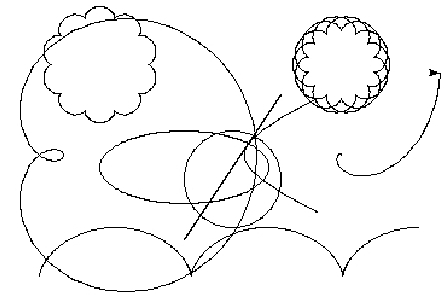
\includegraphics[width=7.5cm]{param2.jpg}$$
\end{fig}
Ecrire une fonction {\tt drawCurve} qui permettent le tracé de telles courbes paramétrées
(figure \ref{fig:traces}).
On utilisera les instructions {\em à la {\sc Logo}} pour réaliser ces tracés
(voir annexe \ref{logo} page \pageref{logo}).
\end{td}
